\documentclass[11pt]{article}

\usepackage[T1]{fontenc}
\usepackage[utf8]{inputenc}
\usepackage{lmodern}
\usepackage[a4paper,margin=1in]{geometry}
\usepackage{amsmath,amssymb,mathtools}
\usepackage{booktabs,longtable,array}
\usepackage{graphicx}
\usepackage{subcaption}
\usepackage{siunitx}
\usepackage{xcolor}
\usepackage{hyperref}
\usepackage{xurl}
\usepackage{float}

\allowdisplaybreaks

\hypersetup{
  colorlinks=true,
  linkcolor=blue!60!black,
  citecolor=blue!60!black,
  urlcolor=blue!60!black,
  pdftitle={Catani--Seymour Subtraction for pp -> t tbar at NLO QCD: A Standalone Implementation}
}

\sisetup{
  round-mode=places,
  round-precision=3,
  scientific-notation=false,
  separate-uncertainty=true,
  table-number-alignment=center
}

\title{Catani--Seymour Subtraction for $pp \to t\bar t$ at NLO QCD:\\A Standalone Implementation}
\author{}
\date{\today}

\begin{document}

\maketitle

\begin{center}
Process: $pp \to t\bar t$ \hspace{1em}
$\sqrt{s}=\SI{8}{TeV}$ \hspace{1em}
PDF set: \texttt{NNPDF31\_nlo\_as\_0118}~\cite{NNPDF31} \hspace{1em}
$\mu_R=\mu_F=m_t$

\vspace{0.5em}
Baseline total-rate configuration: $m_t=\SI{173.3}{GeV}$, $\mu_R=\mu_F=\SI{173.2}{GeV}$

Differential MadGraph-comparison configuration: $m_t=\SI{173.0}{GeV}$, $\mu_R=\mu_F=\SI{173.0}{GeV}$
\end{center}

\begin{abstract}
We document a standalone next-to-leading-order QCD calculation of top-pair production,
$pp \to t\bar t$, at $\sqrt{s}=\SI{8}{TeV}$ based on Catani--Seymour subtraction.
The hadronic cross section is decomposed into Born, real-subtracted, virtual-plus-integrated,
and finite collinear pieces,
\begin{align}
\sigma_{\text{NLO}} = \sigma_{\text{LO}} + \sigma_{\text{RA}} + \sigma_{\text{VA}} + \sigma_{\text{CA}}.
\end{align}
The cleaned package \texttt{cs\_ppttb} contains local analytic Born, virtual, integrated-dipole,
and collinear-counterterm code, with LHAPDF as the only runtime dependency.
In the current release, the inclusive real contribution used by the default run is supplied through a precomputed input,
while the local subtraction framework remains explicit for the other finite NLO pieces.
The subtraction structure, phase-space generation, multichannel integration strategy,
and implementation layout are described in physics terms rather than as a programming manual.
For the inclusive cross section we obtain
$\sigma_{\text{NLO}} = \SI{218.190}{pb} \pm \SI{0.549}{pb}$,
to be compared with the independent reference result
$\sigma_{\text{NLO}} = \SI{218.570}{pb} \pm \SI{0.497}{pb}$.
The difference is $-\SI{0.380}{pb}$, or about $0.17\%$ of the reference rate, and is smaller than the combined Monte Carlo error.
The packaged default run gives a consistent inclusive result, and the available matched-grid
$m_{t\bar t}$ distributions show sensible LO and NLO agreement with MadGraph on the common binning.
\end{abstract}

\section{Introduction}
Top-pair production is one of the most important precision benchmarks at the LHC.
It probes QCD in a kinematic regime with both light and heavy colored partons, it is sensitive to the gluon luminosity,
and it is a standard calibration channel for detector and phenomenological studies.
At leading order the process already receives contributions from both gluon fusion and quark--antiquark annihilation,
but a quantitative description of rates and distributions requires NLO QCD corrections.

The difficulty is familiar: real-emission matrix elements develop soft and collinear singularities,
while one-loop virtual amplitudes contain explicit infrared poles in dimensional regularization.
Neither the real nor the virtual piece is separately finite, even though their sum is finite for an infrared-safe observable.
Any practical NLO calculation must therefore reorganize the perturbative expansion into separately integrable terms.

Catani--Seymour subtraction provides a particularly useful framework for doing so~\cite{Catani:1996vz}.
It introduces local dipole counterterms that reproduce the singular limits of the real matrix element point by point in phase space.
Those dipoles are subtracted from the real contribution and added back after analytic integration over unresolved radiation.
The resulting decomposition yields finite Monte Carlo integrands on Born-like and real-emission phase spaces,
and it provides a systematic bookkeeping of the integrated $I$, $P$, and $K$ operators entering the virtual and collinear sectors.

This report presents the physics setup, the subtraction formulae, the numerical strategy,
and the implementation choices used in the standalone package \texttt{cs\_ppttb}.
The comparison with independent reference calculations is included only to establish the numerical size and stability of the final prediction.
\section{NLO structure}

For an infrared-safe observable $\mathcal{O}$, the NLO hadronic cross section is written as
\begin{align}
\sigma_{\text{NLO}}[\mathcal{O}] &= \sigma_{\text{LO}}[\mathcal{O}] + \sigma_{\text{RA}}[\mathcal{O}] + \sigma_{\text{VA}}[\mathcal{O}] + \sigma_{\text{CA}}[\mathcal{O}],
\end{align}
with
\begin{align}
\sigma_{\text{RA}} &= \int_{\Phi_3} \Bigl[ d\sigma_R - d\sigma_A \Bigr], \\
\sigma_{\text{VA}} &= \int_{\Phi_2} \Bigl[ d\sigma_V + d\sigma_I \Bigr], \\
\sigma_{\text{CA}} &= \int_{\Phi_2} \Bigl[ d\sigma_P + d\sigma_K \Bigr].
\end{align}
The role of each term is as follows.

\begin{itemize}
\item $R$: the full real-emission matrix element on the three-body phase space.
\item $A$: the local Catani--Seymour dipole approximation that reproduces the soft and collinear limits of $R$.
\item $V$: the finite renormalized one-loop contribution on the Born phase space.
\item $I$: the analytically integrated dipole operator whose poles cancel those of the virtual amplitude.
\item $P$ and $K$: the finite initial-state collinear remnants associated with PDF factorization.
\end{itemize}

The standalone package evaluates the hadronic cross section by folding the partonic kernels with PDFs from LHAPDF.
The factorization counterterms are therefore an intrinsic part of the finite hadronic NLO result rather than an optional add-on.
\section{Partonic channels and flavor structure}

At Born level the process is driven by
\begin{align}
gg &\to t\bar t, \\
q\bar q &\to t\bar t,
\end{align}
with $q\in\{u,d,s,c,b\}$.
In the standalone implementation the light-flavor channels are grouped into representative up-type and down-type subprocesses,
while the PDF folding restores the full flavor sum.
The Born representatives are
\begin{align}
gg_{t\bar t},\qquad (d\bar d)_{t\bar t},\qquad (u\bar u)_{t\bar t},\qquad (b\bar b)_{t\bar t}.
\end{align}

The real-emission sector contains
\begin{align}
gg &\to t\bar t g, \\
q\bar q &\to t\bar t g, \\
gq &\to t\bar t q, \\
g\bar q &\to t\bar t \bar q,
\end{align}
again with flavor folding into representative subprocesses.
The real sector is organized into ten representative channels:
\begin{center}
\begin{tabular}{lll}
\path{gg_tt~g} & \path{gd_tt~d} & \path{gu_tt~u} \\
\path{gb_tt~b} & \path{gd~_tt~d~} & \path{gu~_tt~u~} \\
\path{gb~_tt~b~} & \path{dd~_tt~g} & \path{uu~_tt~g} \\
\path{bb~_tt~g} & & \\
\end{tabular}
\end{center}

The PDF luminosities are summed explicitly over the relevant beam directions.
This matters for non-boost-invariant observables such as the pair rapidity $y_{t\bar t}$:
one must include both $q(x_1)\bar q(x_2)$ and $\bar q(x_1)q(x_2)$ contributions to preserve the expected $pp$ symmetry.
\section{Hadronic phase space and Born kinematics}

The hadronic center-of-mass energy is $S=(\sqrt{s})^2$ with $\sqrt{s}=\SI{8}{TeV}$.
The standard variables are
\begin{align}
\tau = x_1 x_2 = \frac{\hat s}{S},
\qquad
Y = \frac{1}{2}\ln\frac{x_1}{x_2},
\end{align}
so that
\begin{align}
x_1 = \sqrt{\tau}\,e^{Y},
\qquad
x_2 = \sqrt{\tau}\,e^{-Y}.
\end{align}
The threshold condition for top-pair production implies
\begin{align}
\tau_{\min} = \frac{4m_t^2}{S},
\qquad
\tau_{\min} \le \tau \le 1,
\qquad
|Y| \le \frac{1}{2}\ln\frac{1}{\tau}.
\end{align}
The Jacobian is simple,
\begin{align}
dx_1\,dx_2 = d\tau\,dY,
\end{align}
and this form is used directly in the hadronic Monte Carlo setup.

For the two-body Born kinematics one may write
\begin{align}
d\Phi_2 = \frac{\beta}{32\pi^2}\,d\cos\theta\,d\phi,
\qquad
\beta = \sqrt{1-\frac{4m_t^2}{\hat s}},
\end{align}
or, after azimuthal integration,
\begin{align}
d\Phi_2 = \frac{\beta}{16\pi}\,d\cos\theta.
\end{align}
Correspondingly,
\begin{align}
\frac{d\hat\sigma_B}{d\cos\theta}
= \frac{\beta}{32\pi\hat s}\,|\mathcal{M}_B|^2,
\end{align}
which is exactly the integrated-azimuth form used by the standalone Born Monte Carlo.
In the code path this appears through the factor
\begin{align}
\texttt{phase\_flux} = \frac{\beta}{32\pi\hat s}.
\end{align}

\section{Real phase space and sampling weights}

The real-emission phase space is generated through Catani--Seymour compatible multichannel mappings.
The phase-space block definitions and channel structure are supplied by the packaged Born and real reference data,
while the local code constructs channel densities $g_c$ for each mapping.
With multichannel weights $\alpha_c$, the combined channel density is
\begin{align}
g_{\text{MC}}(\Phi_3) = \sum_c \alpha_c\,g_c(\Phi_3).
\end{align}
The total sampling density then includes the hadronic variables,
\begin{align}
g_{\text{tot}} = g_{\tau}\,g_{x_1x_2}\,g_{\text{MC}},
\end{align}
and the phase-space weight used by the standalone drivers is
\begin{align}
\texttt{ps\_factor} = \frac{\texttt{hcf}}{g_{\text{tot}}\,\hat s}.
\end{align}
Here \texttt{hcf} collects the fixed normalization and unit-conversion constants needed to return the final result in picobarns.

The same philosophy is used in the Born-like CA and VA integrations, with the appropriate lower-dimensional phase spaces.
For the CA term, additional $z$-variable sampling is introduced because the finite collinear contribution is evaluated on a Born-like phase space augmented by the convolution structure of the $P$ and $K$ kernels.

\section{Catani--Seymour dipoles}

The local counterterm is organized as a sum over dipoles,
\begin{align}
d\sigma_A = \sum_d d\sigma_B \otimes V_d,
\end{align}
where the dipole kernel $V_d$ depends on the emitter--spectator assignment and on the mapped reduced Born configuration.
The implementation covers the standard classes
\begin{align}
\text{FF},\qquad \text{FI},\qquad \text{IF},\qquad \text{II},
\end{align}
distinguishing whether emitter and spectator are in the final or initial state.
With leg labels $1,2$ for the incoming partons, $3=t$, $4=\bar t$, and $5$ for the unresolved real parton, the implemented dipole list is
\begin{center}
\small
\begin{tabular}{>{\raggedright\arraybackslash}p{0.18\textwidth}>{\raggedright\arraybackslash}p{0.74\textwidth}}
\toprule
Real channel & Dipoles and kernels \\
\midrule
$q\bar q\to t\bar t g$ &
\texttt{FF[3,5,4](Qg)}, \texttt{FF[4,5,3](Qg)},
\texttt{FI[3,5,1](Qg)}, \texttt{FI[3,5,2](Qg)}, \texttt{FI[4,5,1](Qg)}, \texttt{FI[4,5,2](Qg)},
\texttt{IF[1,5,3](qg)}, \texttt{IF[1,5,4](qg)}, \texttt{IF[2,5,3](qbg)}, \texttt{IF[2,5,4](qbg)},
\texttt{II[1,5,2](qg)}, \texttt{II[2,5,1](qbg)} \\
$gg\to t\bar t g$ &
\texttt{FF[3,5,4](Qg)}, \texttt{FF[4,5,3](Qg)},
\texttt{FI[3,5,1](Qg)}, \texttt{FI[3,5,2](Qg)}, \texttt{FI[4,5,1](Qg)}, \texttt{FI[4,5,2](Qg)},
\texttt{IF[1,5,3](gg)}, \texttt{IF[1,5,4](gg)}, \texttt{IF[2,5,3](gg)}, \texttt{IF[2,5,4](gg)},
\texttt{II[1,5,2](gg)}, \texttt{II[2,5,1](gg)} \\
$qg\to t\bar t q$ &
\texttt{IF[1,5,3](QQ)}, \texttt{IF[1,5,4](QQ)}, \texttt{IF[2,5,3](gq)}, \texttt{IF[2,5,4](gq)},
\texttt{II[1,5,2](QQ)}, \texttt{II[2,5,1](gq)} \\
$\bar q g\to t\bar t\bar q$ &
\texttt{IF[1,5,3](QBarQBar)}, \texttt{IF[1,5,4](QBarQBar)}, \texttt{IF[2,5,3](gqb)}, \texttt{IF[2,5,4](gqb)},
\texttt{II[1,5,2](QBarQBar)}, \texttt{II[2,5,1](gqb)} \\
$gq\to t\bar t q$ &
\texttt{IF[1,5,3](gq)}, \texttt{IF[1,5,4](gq)}, \texttt{IF[2,5,3](QQ)}, \texttt{IF[2,5,4](QQ)},
\texttt{II[1,5,2](gq)}, \texttt{II[2,5,1](QQ)} \\
$g\bar q\to t\bar t\bar q$ &
\texttt{IF[1,5,3](gqb)}, \texttt{IF[1,5,4](gqb)}, \texttt{IF[2,5,3](QBarQBar)}, \texttt{IF[2,5,4](QBarQBar)},
\texttt{II[1,5,2](gqb)}, \texttt{II[2,5,1](QBarQBar)} \\
\bottomrule
\end{tabular}
\end{center}

The code evaluates every dipole through a common scalar form. For a real momentum point $p$ and its mapped Born point $\tilde p_d$, a dipole contribution is
\begin{align}
D_d(p) =
\frac{8\pi\alpha_s}{N_d}
\left[K_d^{(g)}\,B_d(\tilde p_d)-K_d^{(v)}\,S_d(\tilde p_d;n_d)\right],
\label{eq:local-dipole-master}
\end{align}
where $N_d$ is the dipole normalization denominator, $B_d$ is the color-correlated Born term, and $S_d$ is the spin-correlated Born term. For kernels without a spin term, $K_d^{(v)}=0$. The total local subtraction is
\begin{align}
D(p)=\sum_d D_d(p),
\qquad
R_A(p)=R(p)-D(p).
\end{align}
The symmetry factor multiplying each implemented dipole is one.

The invariant used in the dipole denominator is
\begin{align}
s_{ab}^{\text{code}}=
\begin{cases}
\operatorname{project\_sij}(p_a,p_b), & \text{pair denominator},\\
|\operatorname{matrix\_sij}(p_a,p_b)|, & \text{beam denominator}.
\end{cases}
\end{align}
The Kallen function used in the massive mappings and kernels is
\begin{align}
\lambda(a,b,c)=a^2+b^2+c^2-2ab-2ac-2bc.
\end{align}
The exact kernel formulas used by the real-subtraction construction are the following. For final--final massive $Q\to Qg$ dipoles, with final spectator $k$,
\begin{align}
y_{ij,k} &= \frac{p_i\!\cdot p_j}{p_i\!\cdot p_j+p_i\!\cdot p_k+p_j\!\cdot p_k},
&z_i &= \frac{p_i\!\cdot p_k}{p_i\!\cdot p_k+p_j\!\cdot p_k},\\
\mu_a^2&=\frac{m_a^2}{Q^2},
&Q&=\tilde p_{ij}+\tilde p_k,\\
v_{ij,k}&=
\frac{\sqrt{\left(2\mu_k^2+(1-\mu_i^2-\mu_j^2-\mu_k^2)(1-y_{ij,k})\right)^2-4\mu_k^2}}
{(1-\mu_i^2-\mu_j^2-\mu_k^2)(1-y_{ij,k})},\\
\tilde v_{ij,k}&=
\frac{\sqrt{\lambda(1,\mu_{ij}^2,\mu_k^2)}}{1-\mu_{ij}^2-\mu_k^2},
\end{align}
and
\begin{align}
N_{FF,Qg} &= s_{ij}^{\text{code}}-m_{ij}^2,\\
K^{(g)}_{FF,Qg} &=
\frac{2}{1-z_i(1-y_{ij,k})}
-\frac{\tilde v_{ij,k}}{v_{ij,k}}
\left(1+z_i+\frac{m_{ij}^2}{p_i\!\cdot p_j}\right),
&K^{(v)}_{FF,Qg}&=0.
\end{align}

For final--initial massive $Q\to Qg$ dipoles, with initial spectator $a$,
\begin{align}
1-x_{ij,a} &= \frac{p_i\!\cdot p_j-\frac12(m_{ij}^2-m_i^2-m_j^2)}{p_i\!\cdot p_a+p_j\!\cdot p_a},
&z_i&=\frac{p_i\!\cdot p_a}{p_i\!\cdot p_a+p_j\!\cdot p_a},
&z_j&=\frac{p_j\!\cdot p_a}{p_i\!\cdot p_a+p_j\!\cdot p_a},\\
N_{FI,Qg} &= x_{ij,a}(s_{ij}^{\text{code}}-m_{ij}^2),\\
K^{(g)}_{FI,Qg} &= \frac{2}{1-x_{ij,a}+z_j}-1-z_i-\frac{m_{ij}^2}{p_i\!\cdot p_j},
&K^{(v)}_{FI,Qg}&=0.
\end{align}

For initial--final dipoles, with initial emitter $a$, unresolved parton $i$, and final spectator $k$,
\begin{align}
1-x_{ik,a} &= \frac{p_i\!\cdot p_k}{p_i\!\cdot p_a+p_k\!\cdot p_a},
&u_i&=\frac{p_i\!\cdot p_a}{p_i\!\cdot p_a+p_k\!\cdot p_a},
&N_{IF}&=x_{ik,a}\\,s_{ai}^{\text{code}}.
\end{align}
The scalar kernels are
\begin{align}
K^{(g)}_{IF,qg} &= \frac{2}{1-x_{ik,a}+u_i}-(1+x_{ik,a}),
&K^{(v)}_{IF,qg}&=0,\\
K^{(g)}_{IF,gq} &= \frac{T_R}{C_F}\left[1-2x_{ik,a}(1-x_{ik,a})\right],
&K^{(v)}_{IF,gq}&=0.
\end{align}
For the spin-correlated kernels the polarization vector is
\begin{align}
n_{IF}=\frac{p_i}{u_i}-\frac{p_k}{1-u_i},
\end{align}
and the implemented terms are
\begin{align}
K^{(g)}_{IF,gg} &=2\left[\frac{1}{1-x_{ik,a}+u_i}-1+x_{ik,a}(1-x_{ik,a})\right],\\
K^{(v)}_{IF,gg} &=2 n_{IF}^2\frac{(1-x_{ik,a})u_i(1-u_i)}{x_{ik,a}\,p_i\!\cdot p_k},\\
K^{(g)}_{IF,QQ} &=\frac{C_F}{C_A}x_{ik,a},\\
K^{(v)}_{IF,QQ} &=\frac{C_F}{C_A}n_{IF}^2\frac{2(1-x_{ik,a})u_i(1-u_i)}{x_{ik,a}\,p_i\!\cdot p_k}.
\end{align}
The anti-quark kernels use the same formulas as the corresponding quark kernels.

For initial--initial dipoles, with initial emitter $a$, unresolved parton $i$, and initial spectator $b$,
\begin{align}
x_{i,ab} &= 1-\frac{p_i\!\cdot(p_a+p_b)}{p_a\!\cdot p_b},
&N_{II}&=x_{i,ab}\,s_{ai}^{\text{code}}.
\end{align}
The non-spin kernels are
\begin{align}
K^{(g)}_{II,qg} &= \frac{2}{1-x_{i,ab}}-(1+x_{i,ab}),
&K^{(v)}_{II,qg}&=0,\\
K^{(g)}_{II,gq} &= \frac{T_R}{C_F}\left[1-2x_{i,ab}(1-x_{i,ab})\right],
&K^{(v)}_{II,gq}&=0.
\end{align}
The spin polarization vector and the spin kernels are
\begin{align}
n_{II}&=p_i-p_b\frac{p_a\!\cdot p_i}{p_a\!\cdot p_b},\\
K^{(g)}_{II,gg} &=2\left[\frac{x_{i,ab}}{1-x_{i,ab}}+x_{i,ab}(1-x_{i,ab})\right],\\
K^{(v)}_{II,gg} &=2 n_{II}^2\frac{(1-x_{i,ab})p_a\!\cdot p_b}{x_{i,ab}(p_b\!\cdot p_i)(p_a\!\cdot p_i)},\\
K^{(g)}_{II,QQ} &=\frac{C_F}{C_A}x_{i,ab},\\
K^{(v)}_{II,QQ} &=\frac{C_F}{C_A}n_{II}^2\frac{2(1-x_{i,ab})p_a\!\cdot p_b}{x_{i,ab}(p_a\!\cdot p_i)(p_b\!\cdot p_i)}.
\end{align}

The mapped Born momenta are also explicit. For a final--final dipole, set $P_{ij}=p_i+p_j$, $Q=P_{ij}+p_k$, $P_{ij}^2=m_{P}^2$, $p_k^2=m_k^2$, and use the mapped emitter mass $\tilde m_{ij}^2=p_i^2$. The spectator transverse to $Q$ is
\begin{align}
p_{k\perp}=p_k-Q\frac{Q\!\cdot p_k}{Q^2},
\end{align}
and the mapped momenta are
\begin{align}
\tilde p_k &=
p_{k\perp}\sqrt{\frac{\lambda(Q^2,\tilde m_{ij}^2,m_k^2)}{\lambda(Q^2,m_P^2,m_k^2)}}
+Q\frac{Q^2+m_k^2-\tilde m_{ij}^2}{2Q^2},\\
\tilde p_{ij} &= Q-\tilde p_k.
\end{align}
For a final--initial dipole with incoming spectator $a$,
\begin{align}
x_a &= \frac{p_i\!\cdot p_a+p_j\!\cdot p_a-p_i\!\cdot p_j}{p_i\!\cdot p_a+p_j\!\cdot p_a},\\
\tilde p_a &= x_a p_a,\\
\tilde p_{ij} &= p_i+p_j-(1-x_a)p_a,
\end{align}
while the other incoming momentum and the other final top momentum are unchanged.
For an initial--final dipole with incoming emitter $a$, unresolved parton $i$, and final spectator $k$,
\begin{align}
x_a &= \frac{p_a\!\cdot p_k+p_a\!\cdot p_i-p_k\!\cdot p_i}{p_a\!\cdot p_k+p_a\!\cdot p_i},\\
\tilde p_a &= x_a p_a,\\
\tilde p_k &= p_k+p_i-(1-x_a)p_a,
\end{align}
with the non-emitting incoming momentum and the other final top momentum left unchanged.
For an initial--initial dipole with incoming emitter $a$, unresolved parton $i$, and incoming spectator $b$,
\begin{align}
x_a &= \frac{p_a\!\cdot p_b-p_a\!\cdot p_i-p_i\!\cdot p_b}{p_a\!\cdot p_b},\\
\tilde p_a &= x_a p_a,
\qquad
\tilde p_b=p_b,\\
K&=p_1+p_2-p_i,
\qquad
\tilde K=\tilde p_a+\tilde p_b.
\end{align}
Each final heavy momentum $p_\ell$, $\ell=3,4$, is mapped by
\begin{align}
\tilde p_\ell = p_\ell
- (K+\tilde K)\frac{2p_\ell\!\cdot(K+\tilde K)}{(K+\tilde K)^2}
+ \tilde K\frac{2p_\ell\!\cdot K}{K^2}.
\end{align}

For $pp\to t\bar t$ the final-state top quarks are massive. This modifies the form of the dipole kernels and the kinematic mappings relative to the massless case, in particular in the final-state emitter sectors and in the integrated dipoles entering the $I$ operator. The cleaned standalone implementation packages the dipole metadata in
\path{src/cs_dipole_metadata.cpp}
and the integrated dipole logic in
\path{src/cs_ioperator.cpp}.

\section{Virtual term and the \texorpdfstring{$X$}{X} counterterm}

The virtual contribution is assembled in the form
\begin{align}
\sigma_{\text{VA}} \sim V + X + I.
\end{align}
Here $V$ denotes the finite one-loop virtual correction after ultraviolet renormalization,
$I$ is the integrated Catani--Seymour operator,
and $X$ is the finite UV/renormalization counterterm needed to match the convention used for the reference one-loop amplitudes.

\subsection{Finite integrated \texorpdfstring{$I$}{I} operator}

The finite integrated operator follows the massive Catani--Seymour construction~\cite{Catani:1996vz} and is assembled over ordered color-correlated Born pairs $(i,k)$.
The code uses
\begin{align}
\Delta_1=0,
\qquad
\Delta_2=0,
\qquad
\texttt{switch\_polenorm}=0,
\end{align}
and $N_f=5$ light flavors. The color constants are $C_F=4/3$, $C_A=3$, and $T_R=1/2$. The anomalous dimensions and finite constants are
\begin{align}
\gamma_q &= \frac{3}{2}C_F,
&\gamma_g &= \frac{11}{6}C_A-\frac{2}{3}T_RN_f,\\
K_q &= \left(\frac{7}{2}-\frac{\pi^2}{6}\right)C_F,
&K_g &= \left(\frac{67}{18}-\frac{\pi^2}{6}\right)C_A-\frac{10}{9}T_RN_f.
\end{align}
For each ordered pair the implementation stores the color-correlated Born factor $B_{ik}$ and the positive invariant $s_{ik}$. With
\begin{align}
L_{ik}=\log\frac{\mu_{\text{reg}}^2}{s_{ik}},
\end{align}
the finite contribution from that ordered pair is
\begin{align}
I_{ik}^{\text{fin}} &=-\frac{\alpha_s}{2\pi}\,B_{ik}\,\mathcal{B}_{ik},\\
\mathcal{B}_{ik}
&=\left(VS0_{ik}+VNS_{ik}+F0_i\right)
 +\left(VS1_{ik}+F1_i\right)L_{ik}
 +\frac{1}{2}VS2_{ik}L_{ik}^2,
\end{align}
and
\begin{align}
I^{\text{fin}}=\sum_{(i,k)} I_{ik}^{\text{fin}}.
\end{align}
In the VA kernel $\mu_{\text{reg}}$ is the renormalization scale passed to the virtual sector.

The emitter-dependent finite terms are
\begin{align}
F0_i=
\begin{cases}
-\dfrac{\pi^2}{3}+\dfrac{\gamma_q+K_q}{C_F}+\Delta_1+\dfrac12\log\dfrac{m_t^2}{s_{ik}}-2,
& i \text{ massive},\\[0.9em]
-\dfrac{\pi^2}{3}+\dfrac{\gamma_g+K_g}{C_A},
& i \text{ massless gluon},\\[0.9em]
-\dfrac{\pi^2}{3}+\dfrac{\gamma_q+K_q}{C_F},
& i \text{ massless quark},
\end{cases}
\end{align}
and
\begin{align}
F1_i=
\begin{cases}
\dfrac{-\frac12C_F+\gamma_q}{C_F}, & i \text{ massive},\\[0.7em]
\dfrac{\gamma_g}{C_A}, & i \text{ massless gluon},\\[0.7em]
\dfrac{\gamma_q}{C_F}, & i \text{ massless quark}.
\end{cases}
\end{align}

For a massless emitter and massless spectator,
\begin{align}
VS0&=\Delta_2,
&VS1&=\Delta_1,
&VS2&=1,
&VNS&=0.
\end{align}
Because \texttt{switch\_polenorm} is zero, no additional $-\pi^2/6$ pole-normalization term is added.

For one massive and one massless leg, define
\begin{align}
m^2=m_t^2,
\qquad
Q^2=m^2+s_{ik},
\qquad
\ell_{m/s}=\log\frac{m^2}{s_{ik}},
\qquad
\ell_{s/Q}=\log\frac{s_{ik}}{Q^2},
\qquad
\ell_{m/Q}=\log\frac{m^2}{Q^2}.
\end{align}
Then
\begin{align}
VS0 &= \frac12\Delta_2+\frac12\ell_{m/s}\Delta_1
-\frac14\ell_{m/s}^2-\frac{\pi^2}{12}
-\frac12\ell_{m/s}\ell_{s/Q}
-\frac12\ell_{m/Q}\ell_{s/Q},\\
VS1 &= \frac12\Delta_1+\frac12\ell_{m/s},
&VS2&=\frac12.
\end{align}
If the emitter is the massive quark,
\begin{align}
VNS = \frac{\gamma_q}{C_F}\log\frac{s_{ik}}{Q^2}
+\frac{\pi^2}{6}
-\operatorname{Li}_2\!\left(\frac{s_{ik}}{Q^2}\right)
-2\log\frac{s_{ik}}{Q^2}
-\frac{m^2}{s_{ik}}\log\frac{m^2}{Q^2}.
\end{align}
If the spectator is massive and the emitter is massless,
\begin{align}
VNS = \frac{\gamma_a}{C_a}
\left[
\log\frac{s_{ik}}{Q^2}
-2\log\frac{\sqrt{Q^2}-m_t}{\sqrt{Q^2}}
-\frac{2m_t}{\sqrt{Q^2}+m_t}
\right]
+\frac{\pi^2}{6}
-\operatorname{Li}_2\!\left(\frac{s_{ik}}{Q^2}\right),
\end{align}
where $(\gamma_a,C_a)=(\gamma_g,C_A)$ for a gluon emitter and $(\gamma_q,C_F)$ for a quark emitter.

For two massive legs, define
\begin{align}
Q^2=2m_t^2+s_{ik},
\qquad
\mu_i^2=\mu_k^2=\frac{m_t^2}{Q^2},
\qquad
r_2=\frac{m_t^4}{s_{ik}^2}.
\end{align}
The velocity variable is evaluated as
\begin{align}
v_{ik}=
\begin{cases}
1-\delta,
& r_2<10^{-3},\\[0.4em]
\dfrac{\sqrt{\lambda(1,\mu_i^2,\mu_k^2)}}{1-\mu_i^2-\mu_k^2},
& r_2\ge 10^{-3},
\end{cases}
\end{align}
with
\begin{align}
\delta=
\begin{cases}
2r_2+2r_2^2+4r_2^3+10r_2^4+28r_2^5,
& r_2<10^{-3},\\
1-v_{ik}, & r_2\ge 10^{-3}.
\end{cases}
\end{align}
Next set
\begin{align}
\rho^2 &= \frac{\delta}{1+v_{ik}},
&\log\rho &= \frac12\log\rho^2,\\
\rho_i^2 &=
\frac{1-v_{ik}+\dfrac{2\mu_i^2}{1-\mu_i^2-\mu_k^2}}
{1+v_{ik}+\dfrac{2\mu_i^2}{1-\mu_i^2-\mu_k^2}},
&
\rho_k^2 &=
\frac{1-v_{ik}+\dfrac{2\mu_k^2}{1-\mu_i^2-\mu_k^2}}
{1+v_{ik}+\dfrac{2\mu_k^2}{1-\mu_i^2-\mu_k^2}}.
\end{align}
The singular and non-singular finite pieces are
\begin{align}
VS0 &= \frac{1}{v_{ik}}
\left[
\log\rho\,\Delta_1
-\frac14\log^2\rho_i^2
-\frac14\log^2\rho_k^2
-\frac{\pi^2}{6}
+\log\rho\log\frac{Q^2}{s_{ik}}
\right],\\
VS1 &= \frac{\log\rho}{v_{ik}},
&VS2&=0,
\end{align}
and
\begin{align}
VNS ={}& \frac{\gamma_q}{C_F}\log\frac{s_{ik}}{Q^2}
+\frac{1}{v_{ik}}
\left[
\log\rho^2\log(1+\rho^2)
+2\operatorname{Li}_2(\rho^2)
-\operatorname{Li}_2(1-\rho_i^2)
-\operatorname{Li}_2(1-\rho_k^2)
-\frac{\pi^2}{6}
\right]\\
&+\log\frac{\sqrt{Q^2}-m_t}{\sqrt{Q^2}}
-2\log\frac{(\sqrt{Q^2}-m_t)^2-m_t^2}{Q^2}
-\frac{2m_t^2}{s_{ik}}\log\frac{m_t}{\sqrt{Q^2}-m_t}\\
&-\frac{m_t}{\sqrt{Q^2}-m_t}
+\frac{2m_t(2m_t-\sqrt{Q^2})}{s_{ik}}
+\frac{\pi^2}{2}.
\end{align}

\subsection{Finite \texorpdfstring{$X$}{X} counterterm}

The exact local $X$ term is included explicitly in the local virtual kernel. Define
\begin{align}
L_R=\log\frac{\mu_R^2}{m_t^2},
\qquad
g_s^2=4\pi\alpha_s,
\qquad
\beta=\sqrt{1-\frac{4m_t^2}{\hat s}},
\end{align}
and reconstruct the Born scattering angle from the same invariant used in the code,
\begin{align}
t=\operatorname{project\_sij}(p_1,p_3),
\qquad
c\equiv\cos\theta=\frac{-2m_t^2+\hat s+2t}{\beta\hat s}.
\end{align}
For the quark--antiquark channel,
\begin{align}
X_{q\bar q}=\frac{\alpha_s}{2\pi}
\left[-4C_F-\frac{10}{3}L_R\right]B_{q\bar q}(\hat s,m_t,\mu_R,\alpha_s,c).
\end{align}
For the gluon channel,
\begin{align}
X_{gg}=\frac{\alpha_s}{2\pi}\,g_s^4\left(1+\frac34L_R\right)F^X_{gg}(\beta,c),
\end{align}
with
\begin{align}
F^X_{gg}(\beta,c)=
\frac{1}{9(1-\beta^2c^2)^3}
\Big[&-14\beta^2+23\beta^2c^2
-7\beta^4+17\beta^4c^2-37\beta^4c^4
+14\beta^6-92\beta^6c^2\\
&+146\beta^6c^4-41\beta^6c^6
+50\beta^8c^2-93\beta^8c^4
+43\beta^8c^6-9\beta^8c^8\Big].
\end{align}
The diagnostic decoupling approximation also present in the source is
\begin{align}
X_{\text{dec}}=-2\frac{\alpha_s}{3\pi}T_RL_R\,B,
\end{align}
but the VA kernel uses the exact local formulas above for the reported result.

\section{\texorpdfstring{$P$ and $K$}{P and K} terms and the finite collinear contribution}

Initial-state collinear singularities are factorized into the PDFs. After subtraction and factorization, the finite remnants are organized into the $P$ and $K$ operators,
\begin{align}
\sigma_{\text{CA}} = \int_{\Phi_2} \left[d\sigma_P + d\sigma_K\right].
\end{align}
The $P$ term carries the Altarelli--Parisi splitting-kernel structure tied to PDF factorization,
while the $K$ term completes the finite scheme-dependent remainder of the initial-state subtraction.

In the standalone package there is no separate \texttt{cs\_pk.*} translation unit.
Instead, the finite collinear remnants are evaluated inside
\path{src/cs_ca_integrand.cpp},
which combines the analytic $P$ and $K$ contributions with Born-like phase-space generation and PDF folding.
This is a reasonable packaging choice because the CA contribution is naturally evaluated as a single finite Born-like Monte Carlo integral.

\section{Standalone implementation}

\subsection{Package scope and executable}

The cleaned standalone implementation lives in
\path{cs_ppttb/}.
The main executable is built from
\path{apps/cs_ppttb.cpp}
and installed as
\path{build/bin/cs_ppttb}.
According to the package README and CMake setup, LHAPDF is the only runtime dependency of the final executable.

The package configuration files define the collider energy, masses, scales, PDF choice, event counts, and output locations.
For the default inclusive setup the input is
\path{config/default_8tev.cfg},
which sets
\begin{align}
\sqrt{s} &= \SI{8000}{GeV}, & m_t &= \SI{173.3}{GeV}, & \mu_F = \mu_R &= \SI{173.2}{GeV}.
\end{align}
For the matched-grid MadGraph comparison plots the package uses
\path{config/mtt_madgraph_reference_8tev.cfg},
which adopts $m_t=\mu_F=\mu_R=\SI{173.0}{GeV}$ and a $60$-bin $m_{t\bar t}$ grid from \SI{300}{GeV} to \SI{1000}{GeV}.

\subsection{Module map}

The cleaned standalone package is not organized as a monolithic integrator.
Instead, the physics responsibilities are split across a compact set of focused modules:

\begin{center}
\begin{tabular}{p{0.28\textwidth}p{0.62\textwidth}}
\toprule
Module(s) & Role \\
\midrule
\path{cs_phasespace.*} & Born and mapped phase-space generation, channel blocks, and densities. \\
\path{born.cpp}, \path{virtual.cpp}, \path{real.hpp} & Local analytic Born and finite virtual building blocks, plus real-channel definitions used by the standalone workflow. \\
\path{color_correlation.*}, \path{cs_born_correlations.*} & Color-correlated Born structures needed by dipoles and integrated operators. \\
\path{cs_dipole_metadata.*} & Typed description of Catani--Seymour dipole channels and mappings. \\
\path{cs_ioperator.*} & Integrated dipole operator entering the virtual sector. \\
\path{cs_ct_shift.*}, \path{cs_va_kernel.*}, \path{cs_va_integrand.*} & Finite virtual assembly, exact local $X$ counterterm, and the final VA integrand. \\
\path{cs_ca_integrand.*} & Finite $P$ and $K$ collinear remnants evaluated on Born-like phase space. \\
\path{cs_histogram.hpp} & Histogram accumulation and finalization. \\
\path{cs_runner.*} & Monte Carlo orchestration, PDF folding, observable definitions, output writing. \\
\path{cs_config.*} & Parsing and consistency checks for run configuration files. \\
\path{cs_plot.*} & Lightweight internal plotting for package-produced histograms. \\
\bottomrule
\end{tabular}
\end{center}

The package evaluates the Born, virtual, and collinear pieces locally. For the default inclusive run, the real contribution is read from a precomputed input declared in the configuration. When a matched real-emission histogram is supplied through \texttt{ra\_histogram\_csv}, the same framework can assemble differential NLO distributions.

\section{Monte Carlo integration strategy}

All components are evaluated by straightforward Monte Carlo averaging over generated trials,
\begin{align}
I_N = \frac{1}{N}\sum_{i=1}^N w_i,
\qquad
\Delta I_N = \sqrt{\frac{\mathrm{Var}(w)}{N}}.
\end{align}
The variance estimate is built from the usual unbiased sample estimator. The normalization is based on generated trials rather than only accepted events. In the real sector this keeps the Monte Carlo normalization aligned with the channel generation procedure, including the technically singular trials that are rejected by construction.

For the real-emission part the accepted-event count is tracked separately from the generated-trial count.
In a representative inclusive run, the real sector uses $10^6$ generated trials with $994160$ accepted events. The CA and VA integrations are performed on Born-like phase spaces and therefore have unit acceptance in the corresponding sampling variables.

Independent subprocesses are integrated separately and the total uncertainty is formed by quadrature,
\begin{align}
\Delta\sigma_{\text{tot}} = \sqrt{\sum_a (\Delta\sigma_a)^2},
\end{align}
which is the convention used throughout the numerical results quoted below.

\section{Results}

\subsection{Inclusive cross section}

The inclusive prediction is compared with an independent MATRIX calculation~\cite{MATRIX} in Table~\ref{tab:inclusive-components}. All results are quoted in pb. The agreement is good for each separate component and for the final sum. For the total NLO rate, the difference is $-\SI{0.380}{pb}$, which is only $0.17\%$ of the reference value and is smaller than the combined Monte Carlo error, $\SI{0.740}{pb}$.

\begin{table}[H]
\centering
\caption{Inclusive contributions to $pp\to t\bar t$ at $\sqrt{s}=\SI{8}{TeV}$.}
\label{tab:inclusive-components}
\begin{tabular}{lrrrr}
\toprule
Component & Local [pb] & MATRIX [pb] & Difference [pb] & Combined error [pb] \\
\midrule
LO & $147.766 \pm 0.390$ & $147.924 \pm 0.316$ & $-0.158$ & $0.502$ \\
RA & $-5.272 \pm 0.124$ & $-5.198 \pm 0.123$ & $-0.074$ & $0.175$ \\
CA & $88.683 \pm 0.364$ & $88.865 \pm 0.362$ & $-0.182$ & $0.513$ \\
VA & $-12.988 \pm 0.027$ & $-13.021 \pm 0.027$ & $0.033$ & $0.038$ \\
NLO total & $218.190 \pm 0.549$ & $218.570 \pm 0.497$ & $-0.380$ & $0.740$ \\
\bottomrule
\end{tabular}
\end{table}

The VA contribution deserves special attention because it combines the finite one-loop remainder, the integrated dipoles, and the finite counterterm $X$. The numerical stability of that sector is essential for the stability of the full prediction, and the table shows that it is under good control.

The packaged default inclusive run gives
\begin{align}
\sigma_{\text{NLO}}^{\text{pkg}} = \SI{218.667}{pb} \pm \SI{0.549}{pb},
\end{align}
which is consistent with the local assembly above.

\subsection{Differential \texorpdfstring{$m_{t\bar t}$}{mttbar} distribution}

The differential study uses a matched MadGraph5\_aMC@NLO grid~\cite{MG5} with $m_t=\mu_F=\mu_R=\SI{173.0}{GeV}$ and $60$ bins in the range
\begin{align}
m_{t\bar t}\in[\SI{300}{GeV},\SI{1000}{GeV}].
\end{align}
On this interval the integrated local rates are
\begin{align}
\sigma_{\text{LO}}^{300\text{--}1000} &\approx \SI{149.025}{pb}, \\
\sigma_{\text{NLO}}^{300\text{--}1000} &\approx \SI{220.599}{pb}.
\end{align}

\begin{figure}[p]
  \centering
  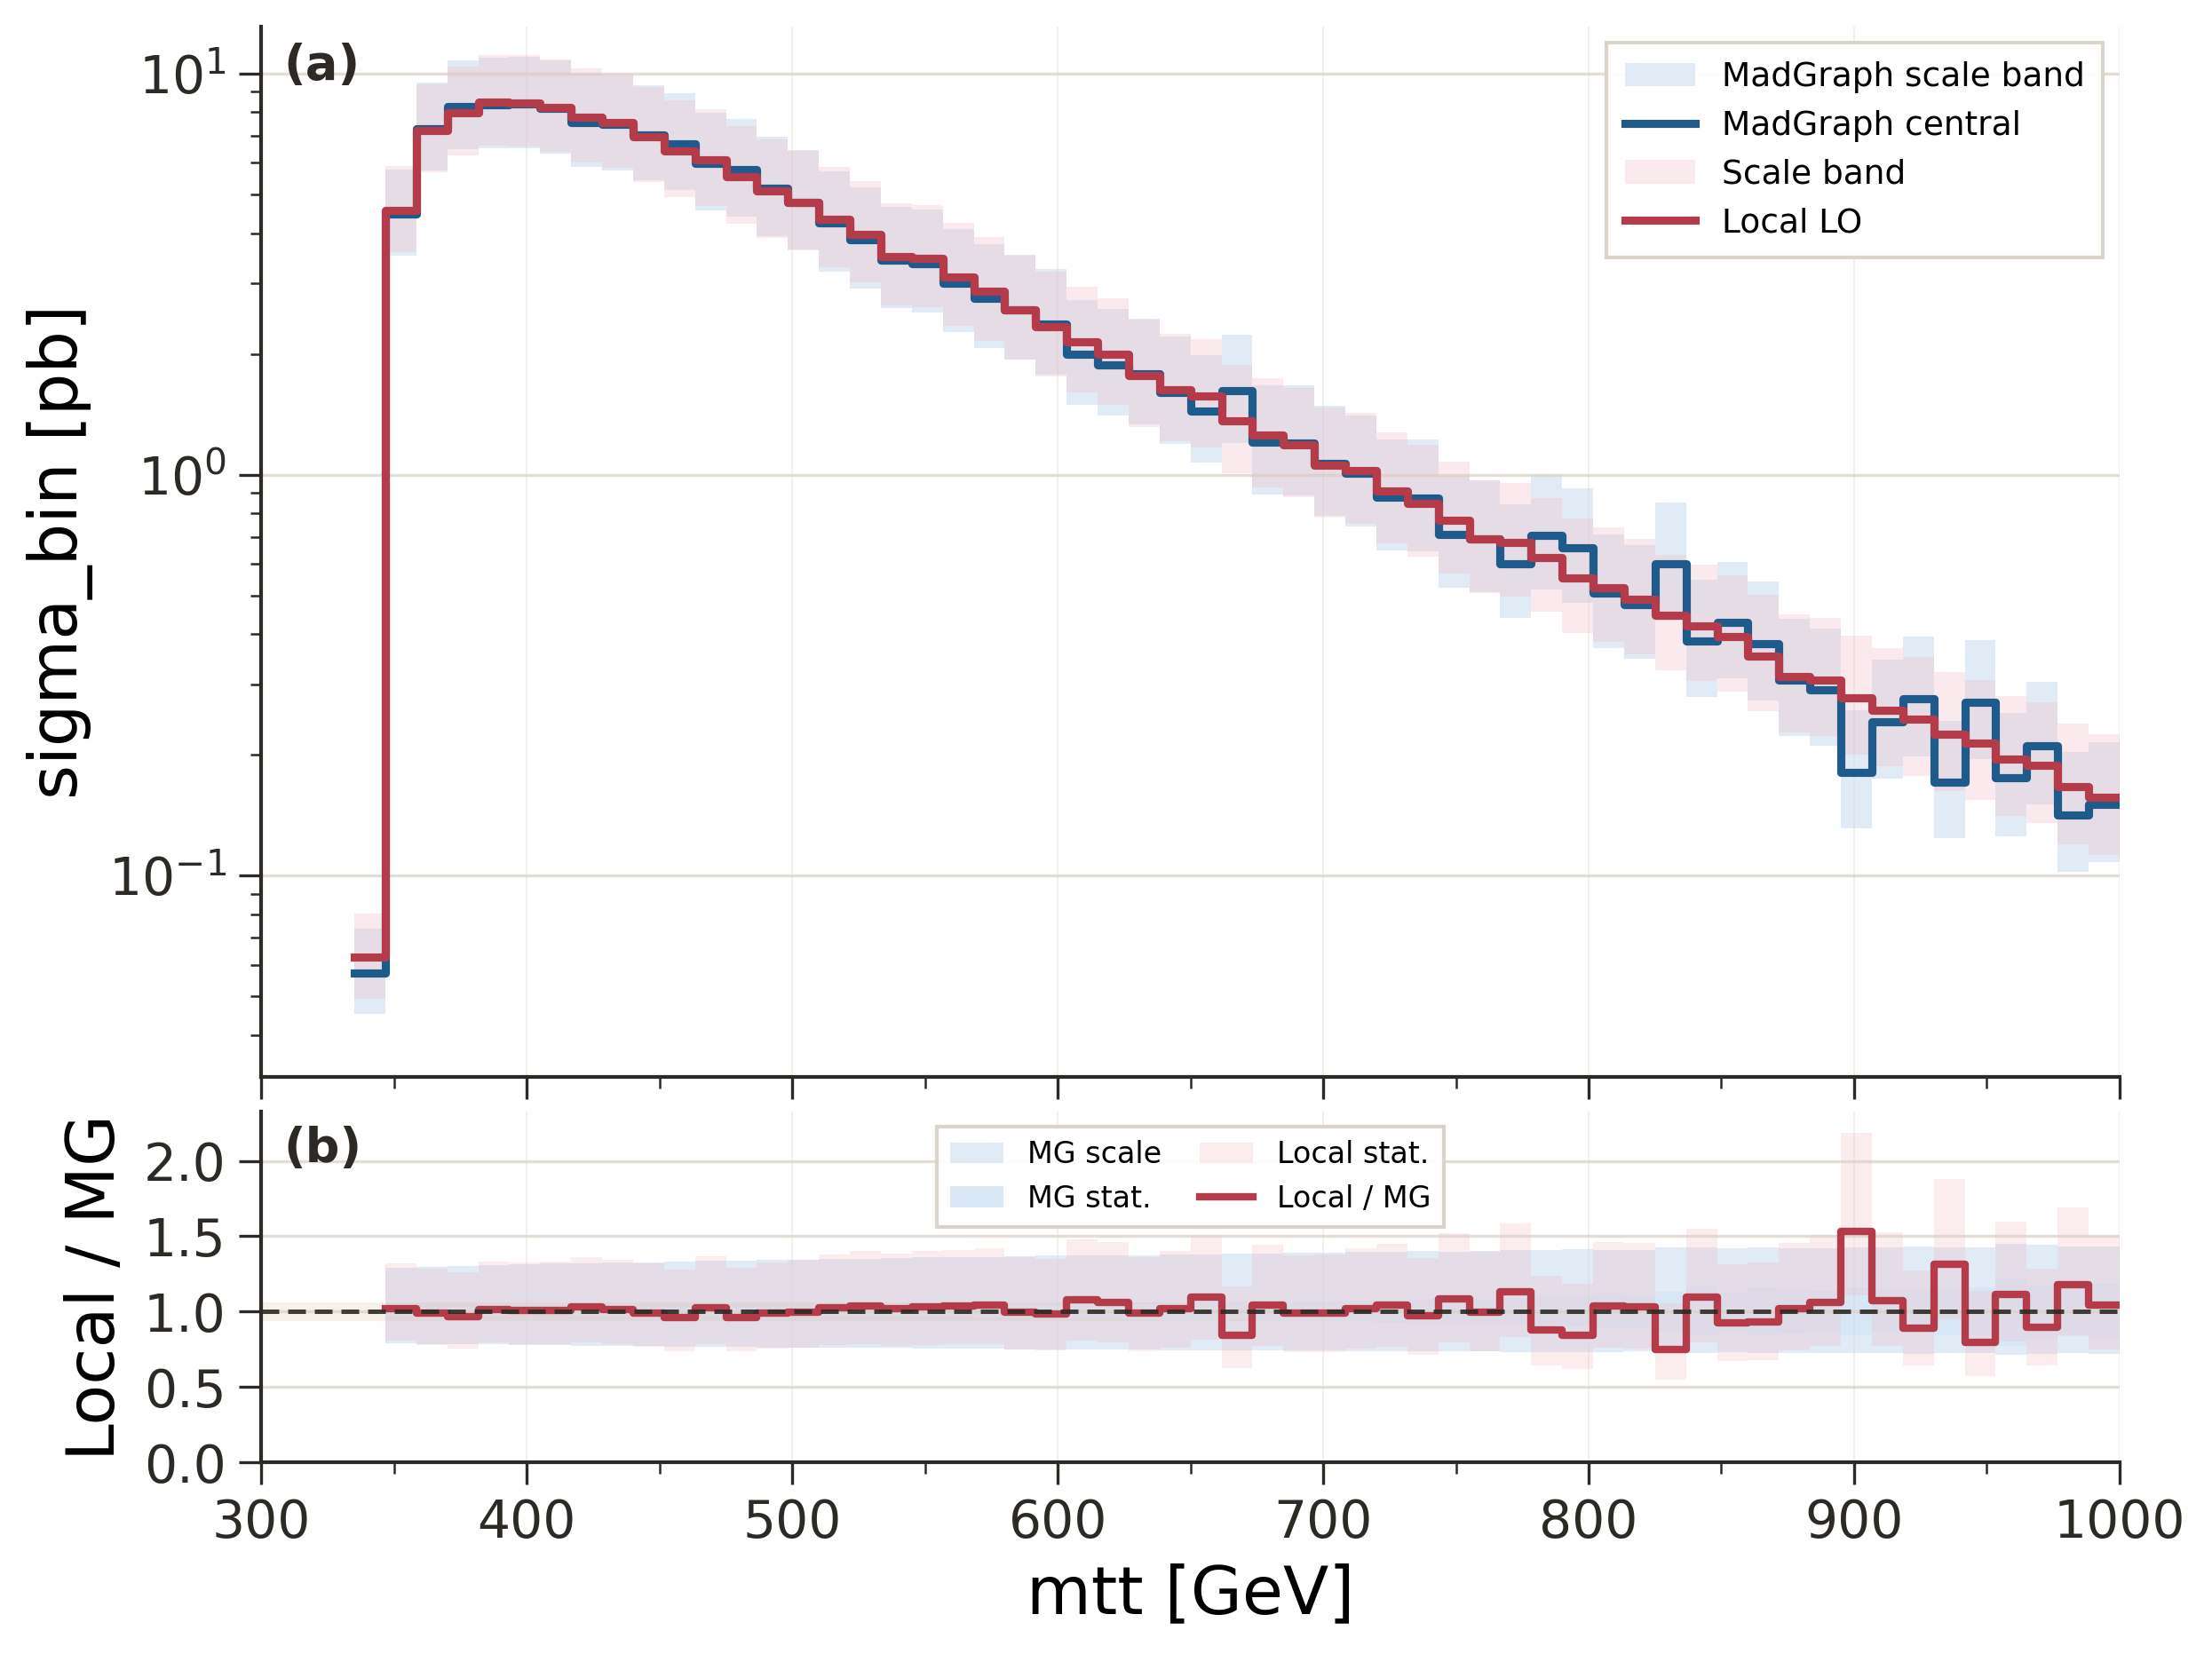
\includegraphics[width=0.92\textwidth]{../results/mtt_madgraph_reference_8tev/plots/python/mtt_lo_vs_madgraph.png}
  \caption{LO invariant-mass distribution for $pp\to t\bar t$ at $\sqrt{s}=\SI{8}{TeV}$ on the matched $60$-bin grid. The shaded band is the scale envelope from $\mu=m_t/2$, $m_t$, and $2m_t$.}
  \label{fig:mtt-lo}
\end{figure}

\begin{figure}[p]
  \centering
  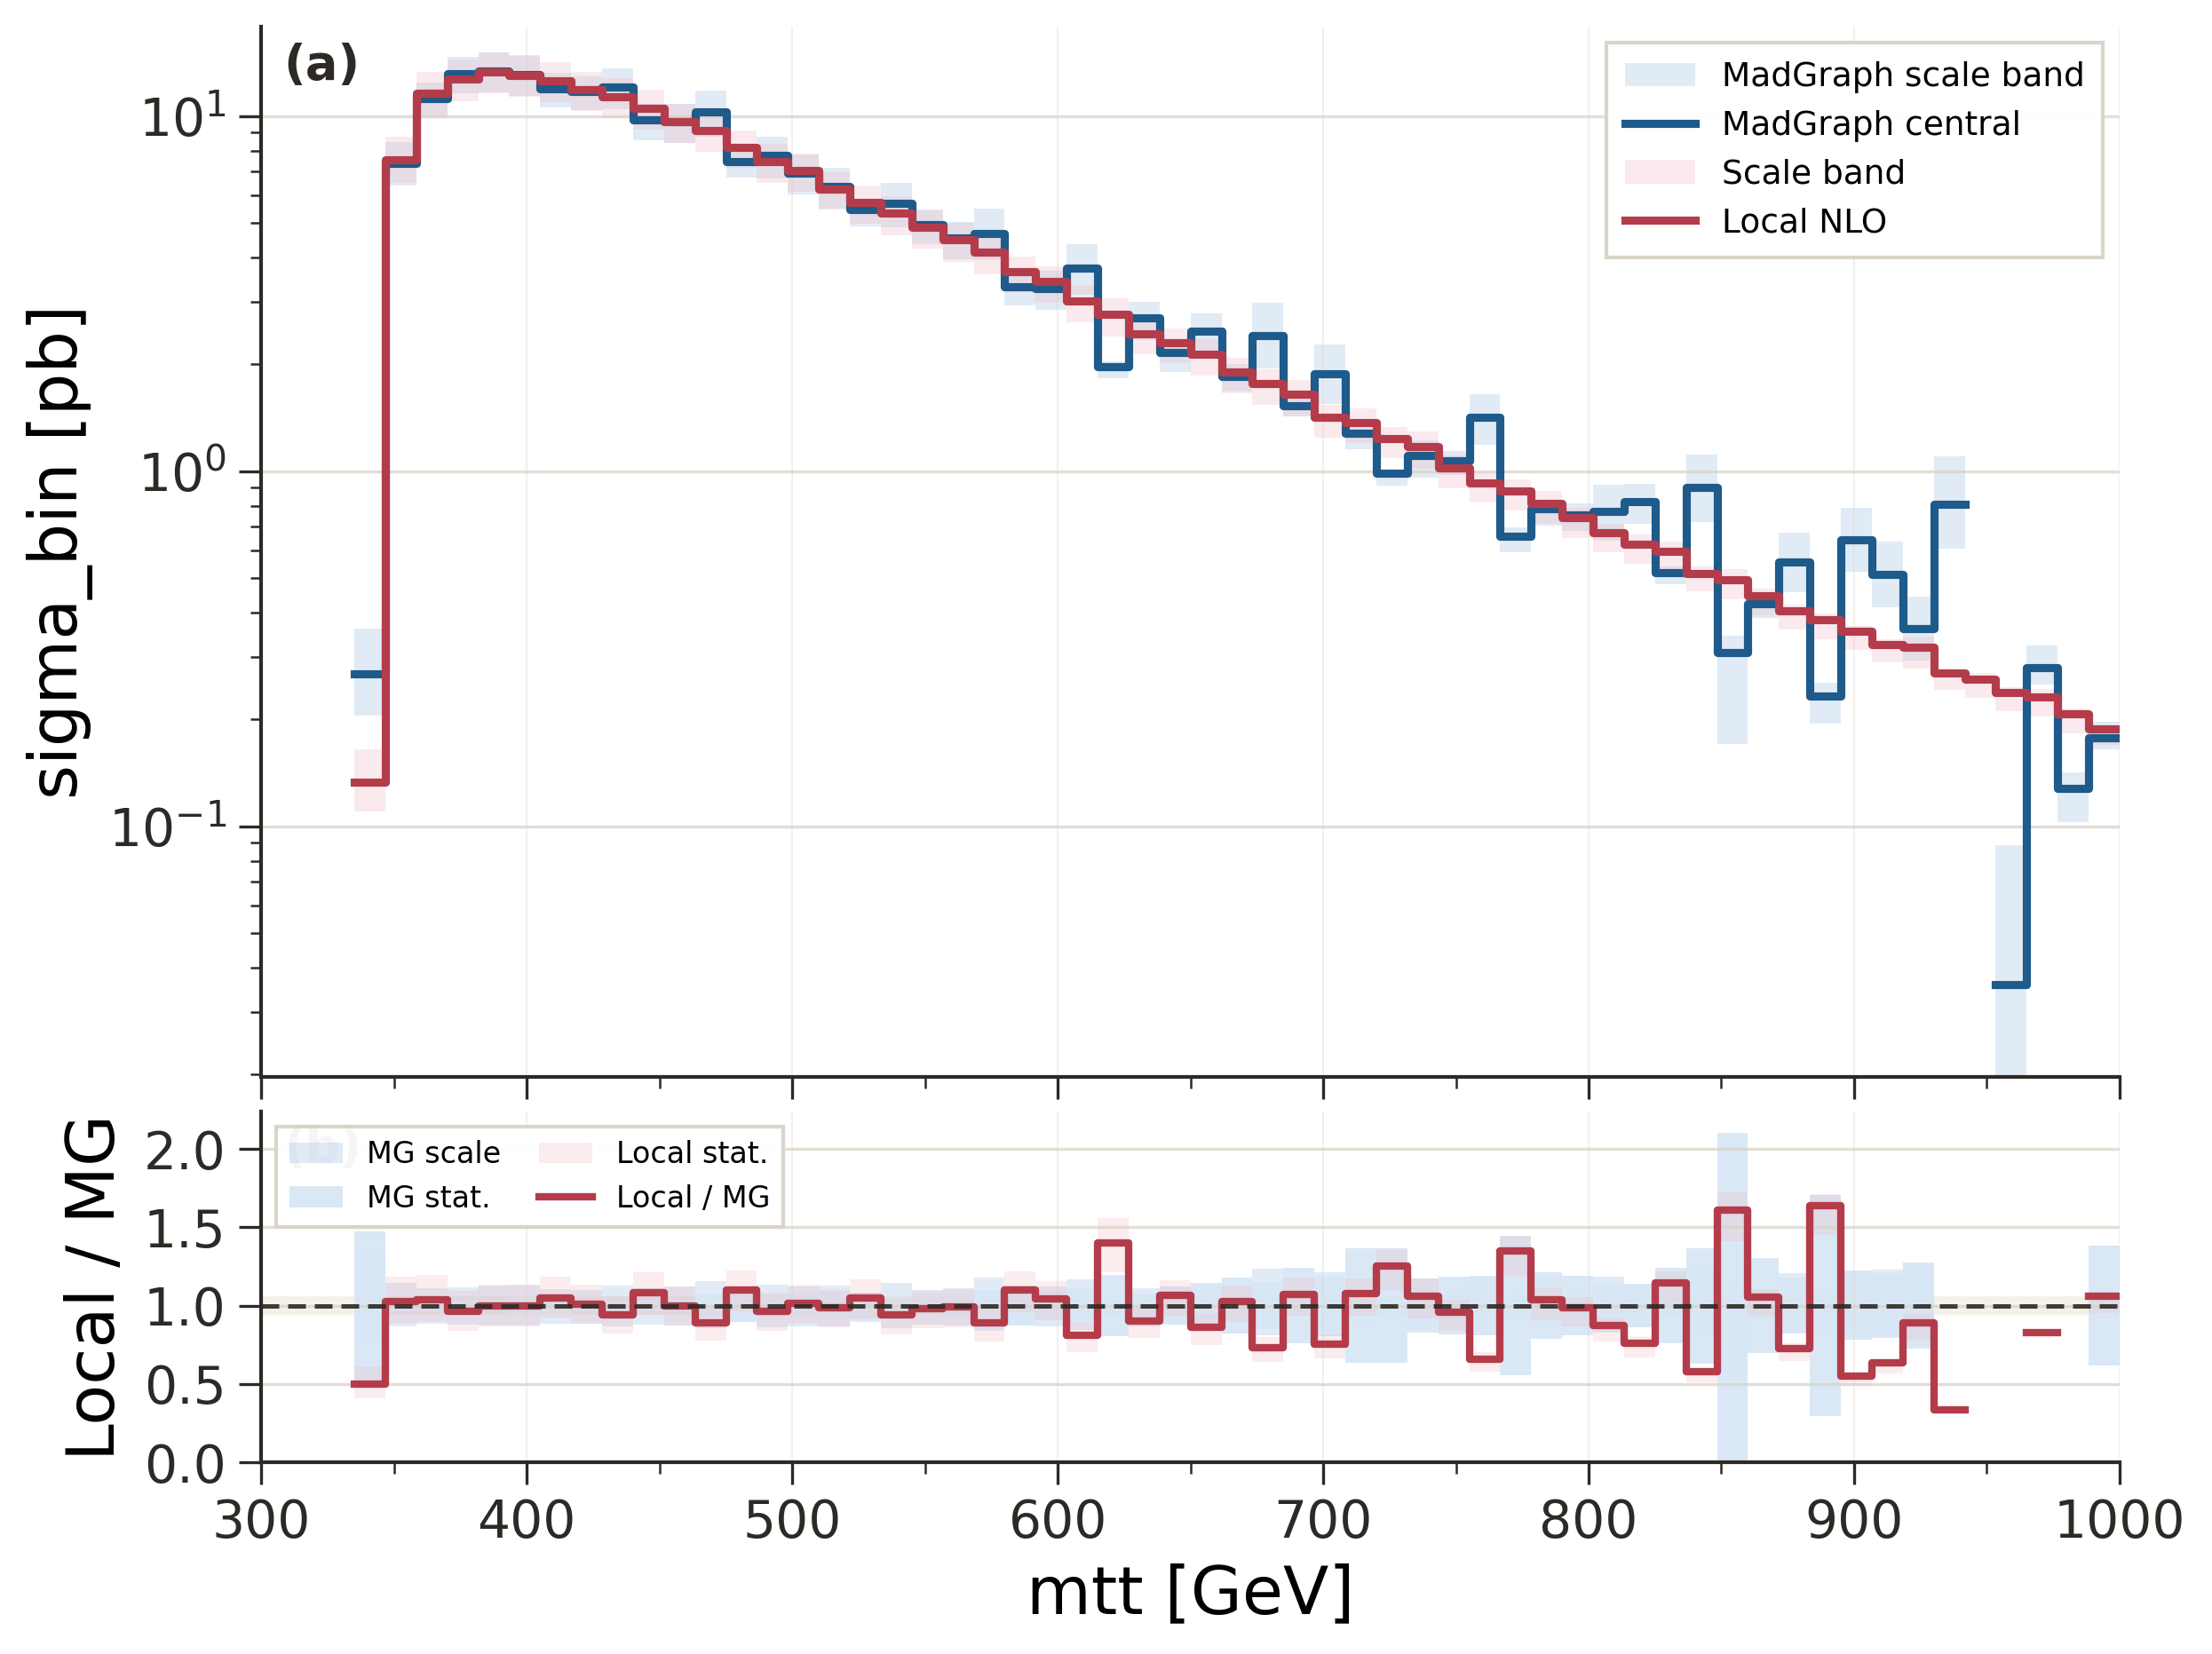
\includegraphics[width=0.92\textwidth]{../results/mtt_madgraph_reference_8tev/plots/python/mtt_nlo_vs_madgraph.png}
  \caption{NLO invariant-mass distribution on the same grid. The local histogram is assembled from LO, RA, CA, and VA contributions using the matched real-emission histogram on this binning.}
  \label{fig:mtt-nlo}
\end{figure}

The LO and NLO shapes follow the MadGraph reference closely across the full range shown here. This is the natural differential counterpart of the inclusive comparison in Table~\ref{tab:inclusive-components}: once the real contribution is available on the target grid, the subtraction framework remains numerically stable for a nontrivial observable.

\section{Discussion}

Three points stand out.

First, the inclusive NLO rate is numerically stable and agrees well with the independent reference calculation. The component-by-component agreement shows that the cancellation of infrared singularities is working as intended in the assembled hadronic prediction.

Second, the package is genuinely standalone at runtime, but the default inclusive setup does not yet generate the real contribution on the fly. Instead, that term is supplied as a precomputed input. This keeps the executable simple and makes the present scope of the package clear.

Third, the differential results show that the same subtraction framework extends smoothly from total rates to distributions. The $m_{t\bar t}$ comparison is therefore more than a visual cross-check: it confirms that the finite NLO pieces combine correctly on a fixed histogram grid.

Natural extensions of the present work include higher-statistics runs, a fully local spin-correlated real-emission kernel inside \texttt{cs\_ppttb}, improved adaptive importance sampling, and a broader set of differential observables.

\section{Conclusion}

We have described a standalone Catani--Seymour subtraction calculation for $pp\to t\bar t$ at NLO QCD at $\sqrt{s}=\SI{8}{TeV}$.
The calculation is organized into Born, real-subtracted, virtual-plus-integrated, and finite collinear sectors, and the package \texttt{cs\_ppttb} implements the local ingredients needed for the Born, VA, and CA pieces while allowing the full NLO prediction to be assembled in a clean runtime environment.

For the inclusive rate we find
\begin{align}
\sigma_{\text{NLO}} = \SI{218.190}{pb} \pm \SI{0.549}{pb},
\end{align}
to be compared with the reference value
\begin{align}
\sigma_{\text{NLO}}^{\text{MATRIX}} = \SI{218.570}{pb} \pm \SI{0.497}{pb}.
\end{align}
The difference is smaller than the combined Monte Carlo uncertainty. The matched-grid $m_{t\bar t}$ distributions also show good agreement with MadGraph at LO and NLO.

These results show that the Catani--Seymour calculation of $pp\to t\bar t$ has been implemented in a compact standalone package with a clear physics structure and reliable numerical behavior.

\appendix

\section{Jacobian and weight formulas}

The hadronic variables satisfy
\begin{align}
x_1 = \sqrt{\tau}\,e^Y,
\qquad
x_2 = \sqrt{\tau}\,e^{-Y},
\end{align}
with Jacobian
\begin{align}
\left|\frac{\partial(x_1,x_2)}{\partial(\tau,Y)}\right| = 1,
\qquad
dx_1\,dx_2 = d\tau\,dY.
\end{align}
After azimuthal integration, the Born-level partonic differential cross section is implemented as
\begin{align}
\frac{d\hat\sigma_B}{d\cos\theta} = \frac{\beta}{32\pi\hat s}|\mathcal{M}_B|^2,
\end{align}
and the Monte Carlo event weight is obtained by dividing by the sampling density,
\begin{align}
w_i = \frac{f_i}{g_i}.
\end{align}
For the real-emission integrator the phase-space factor is stored as
\begin{align}
\texttt{ps\_factor} = \frac{\texttt{hcf}}{g_{\text{tot}}\,\hat s}.
\end{align}

\section{Representative subprocess tables}

\begin{table}[H]
\centering
\caption{Representative subprocess organization used in the standalone implementation.}
\begin{tabular}{ll}
\toprule
Sector & Representatives \\
\midrule
Born/CA/VA & $gg_{t\bar t}$, $(d\bar d)_{t\bar t}$, $(u\bar u)_{t\bar t}$, $(b\bar b)_{t\bar t}$ \\
Real/RA & $gg\to t\bar t g$, $q\bar q\to t\bar t g$, $gq\to t\bar t q$, $g\bar q\to t\bar t\bar q$ \\
Flavor folding & down-type, up-type, and bottom representatives with explicit PDF sums \\
\bottomrule
\end{tabular}
\end{table}

\begin{thebibliography}{99}

\bibitem{Catani:1996vz}
S.~Catani and M.~H.~Seymour,
``A General algorithm for calculating jet cross sections in NLO QCD,''
Nucl. Phys. B \textbf{485} (1997) 291--419,
\href{https://arxiv.org/abs/hep-ph/9605323}{hep-ph/9605323}.

\bibitem{MG5}
J.~Alwall \textit{et al.},
``The automated computation of tree-level and next-to-leading order differential cross sections, and their matching to parton shower simulations,''
JHEP \textbf{07} (2014) 079,
\href{https://arxiv.org/abs/1405.0301}{arXiv:1405.0301}.

\bibitem{NNPDF31}
R.~D.~Ball \textit{et al.},
``Parton distributions from high-precision collider data,''
Eur. Phys. J. C \textbf{77} (2017) 663,
\href{https://arxiv.org/abs/1706.00428}{arXiv:1706.00428}.

\bibitem{MATRIX}
M.~Grazzini, S.~Kallweit and M.~Wiesemann,
``Fully differential NNLO computations with MATRIX,''
Eur. Phys. J. C \textbf{78} (2018) 537,
\href{https://arxiv.org/abs/1711.06631}{arXiv:1711.06631}.

\end{thebibliography}

\end{document}